\begin{figure}[H]
    \centering
    \caption{Distribuição de Trabalhos Relacionados à Computação em IOT}
    \label{fig:dist_trab_rel_comp_iot}
  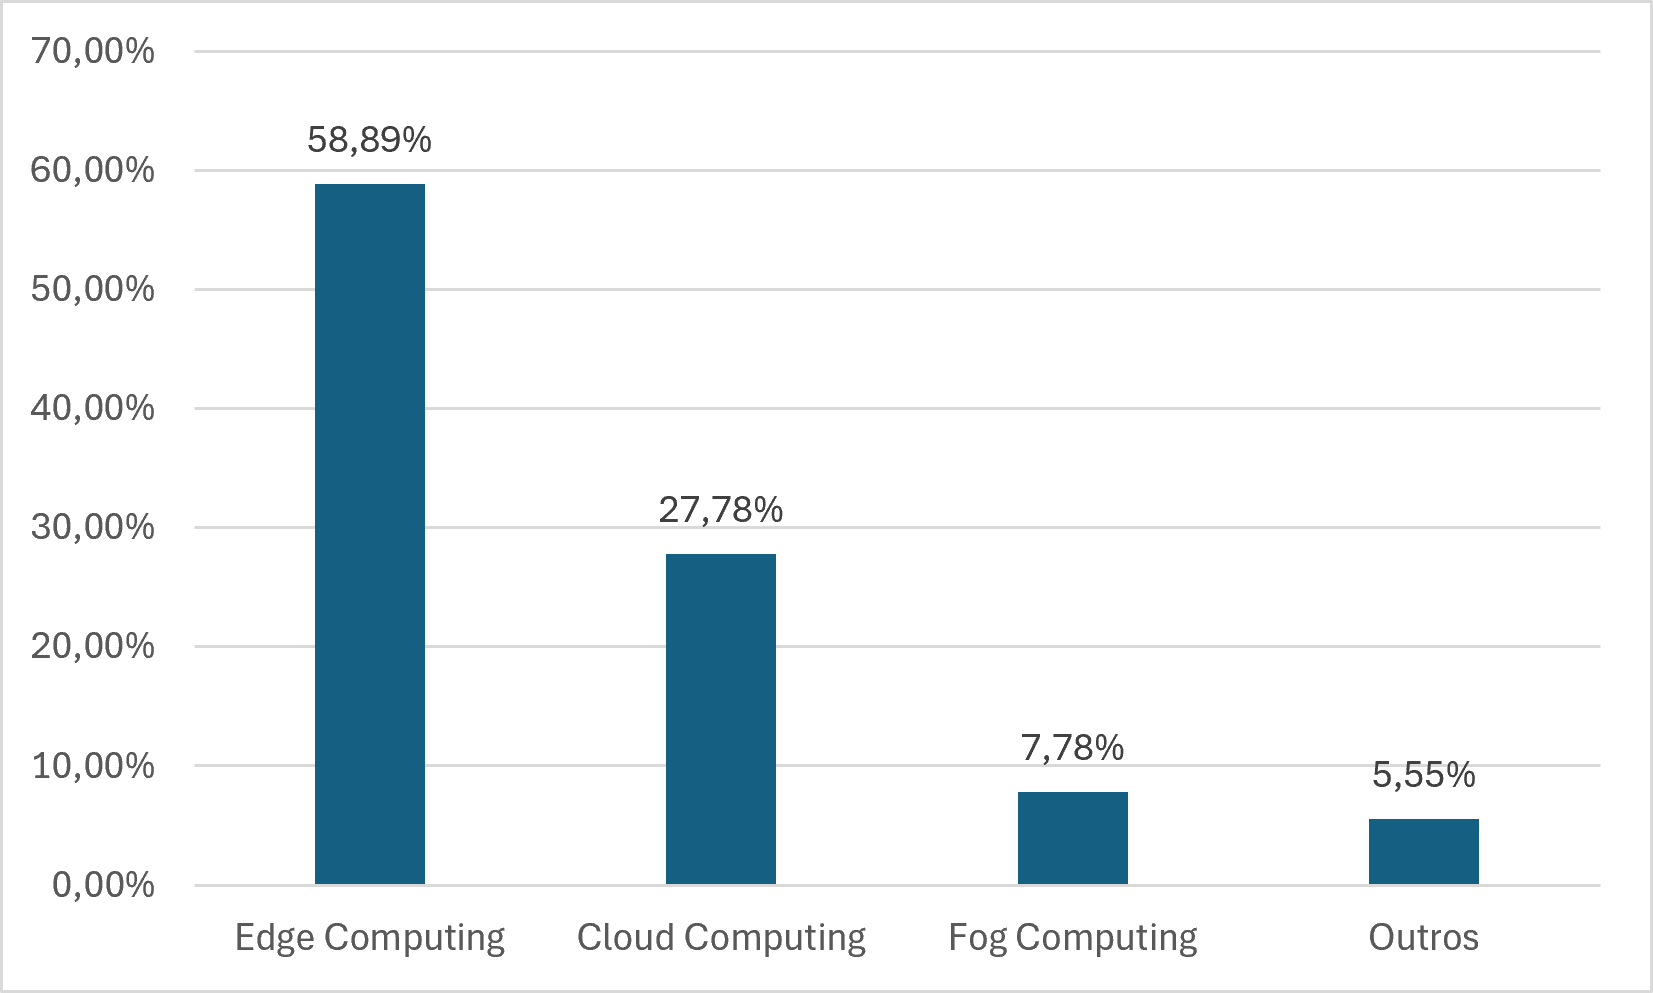
\includegraphics[width=0.85\textwidth]{sections/imagens/trabalhos_relacionados_cloud_edge_computing.png}
    \small
    \begin{quote}
        Fonte: Adaptado de \citeonline{andriulo2024edge}.
    \end{quote}
\end{figure}

\gls{edge_computing} (computação em borda), 
em \gls{iot} é uma arquitetura baseada em processamento descentralizado de dados,
onde ocorre o processamento com o objetivo de construção de informações à 
partir de dispositivos que tem por responsabilidade inicial a 
extração de dados do ambiente real. Como explicado por \citeonline{andriulo2024edge}, 
o gráfico apresentado na figura~\ref{fig:dist_trab_rel_comp_iot} demonstra que 
\gls{edge_computing} é a abordagem mais amplamente difundida na literatura, 
sendo uma solução voltada à segurança de informações, otimização de redes 
de baixa largura de banda e promovendo possível redução de custos operacionais. 

\gls{cloud_computing} (computação em nuvem), ainda no ambiente \gls{iot} 
é um tipo de arquitetura pautado pela alta escalabilidade de armazenamento 
de dados e poder computacional centralizado ou não. 
Como explicado também por \citeonline{andriulo2024edge}, 
este tipo de arquitetura têm como prós a possível adoção de provedores de nuvem,
acoplando serviços como \gls{iaas}, \gls{saas}, entre outros, 
assim reduzindo investimentos iniciais, apresentando maior facilidade de manutenção 
sistêmica e menor complexidade no desenvolvimento de firmware.

\begin{table}[H] 
    \centering     
    \caption{Vantagem e Desvantagens na Adoção de Métodos de Processamento}
    \label{tab:vant_desvant_edge_cloud}
    \begin{tabular}{|c|c|c|} 
    \hline 
    \textbf{Método} & \textbf{Vantagens} & \textbf{Desvantagens} \\ 
    \hline 
        Edge Computing & 
        Menor latência na transmissão de mensagens;
        Menor tráfego de mensagens em rede;
        Foco em segurança de dados & 
        Possível altos custos iniciais;
        Capacidade computacional limitada;
        Dificuldades de execução de modelos de machine learning;
        Dificuldades em escalabilidade; \\
    \hline 
        Cloud Computing & 
        Maior poder computacional disponível;
        Escalabilidade;
        Possível menor custo inicial; & 
        Alta latência;
        Maior risco em segurança de dados;
        Maior quantidade de pacotes enviados à rede; \\ 
    \hline 
    \end{tabular} 
    \begin{quote}
        Fonte: Adaptado de \citeonline{andriulo2024edge}.
    \end{quote}
\end{table} 

A tabela~\ref{tab:vant_desvant_edge_cloud}, 
explícita que tanto \gls{cloud_computing} quanto \gls{edge_computing}, 
trazem prós e contras em relação à sua implementação em projetos. 
Cada projeto tem uma necessidade à ser suprida, e não se atentar à nuances 
do processo de modelagem sistêmica pode acarretar em absorver desvantagens em que 
o projeto não está preparado para lidar.